\newcommand{\mytitle}{From Determinacy to Woodins}
%\input{/home/leidem/Dropbox/std_preamble.tex}
%\input{/home/leidem/Dropbox/art.tex}
\input{/Users/dn16382/Dropbox/std_preamble.tex}
\input{/Users/dn16382/Dropbox/art.tex}

\abstract{
	We give the main ideas in the proof of $\Theta^{L(\mathbb R)}$ being Woodin in $\hod^{L(\mathbb R)}$ assuming $\ad$, due to Woodin. We first give a full proof of Solovay's theorem of the measurability of $(\bf\delta^1_1)^{L(\mathbb R)}=\omega_1^V$ in $L(\mathbb R)$, then sketch how the same ideas generalises to $(\bf\delta^2_1)^{L(\mathbb R)}$, and lastly show how (essentially) the same techniques are used to show Woodin's theorem. This is following \cite{KoellnerWoodin}.
}

The main goal for this note is to describe what ideas are used in the proof of the following theorem.

\theo[Woodin]{
	Assume $\zf+\dc+\ad$. Then
	\eq{
		\hod^{L(\mathbb R)}\models\Theta^{L(\mathbb R)}\text{ is a Woodin cardinal}.
	}
}

It should be noted that the theorem \textit{can} be proven without using $\dc$ by using an equivalent definition of Woodin cardinals, but that's not the goal here. We will use the following definition of Woodin cardinals.

\defi{
	A cardinal $\delta$ is \textbf{Woodin} if given any $A\subset\delta$ there is a cardinal $\kappa<\delta$ which is $A$-reflecting; that is, to every $\lambda<\delta$ there is an elementary embedding
	\eq{
		j_\lambda:V\to\M
	}

	with $\crit j_\lambda=\kappa$, $j_\lambda(\kappa)>\lambda$, $V_\lambda\subset\M$ and $j_\lambda(A)\cap\lambda=A\cap\lambda$.
}

We're going to show Woodin's theorem in a series of steps. We first aim to show that $(\bf\delta^2_1)^{L(\mathbb R)}$ is measurable in $\hod^{L(\mathbb R)}$, and as a warm-up we'll show that $(\bf\delta^1_1)^{L(\mathbb R)}=\omega_1^V$ is measurable in $L(\mathbb R)$. These two results will turn out to use essentially the same techniques as the ones used in the proof of the main theorem. Before we describe these techniques we'll delve straight into the proof of $\omega_1$ being measurable in $L(\mathbb R)$ -- that'll make it easier to 'generalise' the ideas used to the other results.


\section{First warm-up: measurability of $\omega_1$}

Before we start the proof we need to introduce some terminology. For $x\in\r$ define the binary relation
\eq{
	E_x:=\{(m,n)\in\omega\times\omega\mid x(\bra{m,n})=0\},
}

where $\bra{\cdot,\cdot}:\omega\times\omega\to\omega$ is a recursive bijection. Then the key set is the following:
\eq{
	\wo:=\{x\in\r\mid E_x\text{ is a wellordering}\}.
}

Also, setting $\alpha_x$ to be the order-type of $E_x$, set $\wo_\alpha:=\{x\in\wo\mid\alpha_x=\alpha\}$ and define $\wo_{<\alpha}$, $\wo_{\leq\alpha}$ and $\wo_{[\alpha,\beta]}$ and so on in the obvious fashion. The essential properties of $\wo$ are the following two results.

\qlemm[$\b\Sigma^1_1$-Boundedness; Luzin-Sierpinski]{
	Assume $\zf+\ac_\omega(\mathbb R)$. Then whenever $X\subset\wo$ is $\b\Sigma^1_1$ there is some $\alpha<\omega_1$ such that $X\subset\wo_{<\alpha}$.
}

\qlemm[Basic Coding; Solovay]{
	Assume $\zf+\ad$ and let $Z\subset\wo\times\r$. Then there is a $\b\Sigma^1_2$ subset $Z^*\subset Z$ such that $Z^*$ is a \textbf{selector} for $Z$, i.e. that for every $\alpha<\omega_1$ it holds that
	\eq{
		Z^*\cap(\wo_\alpha\times\r)\neq\emptyset\Leftrightarrow Z\cap(\wo_\alpha\times\r)\neq\emptyset.
	}

	Furthermore, we can choose $Z^*$ to be of the form $X\cap(\wo\times\r)$, where $X\subset\r\times\r$ is $\b\Sigma^1_1$.
}

See Figure \ref{fig.coding1} for an illustration of Basic coding. The proof of the $\b\Sigma^1_1$-Boundedness is essentially that if $X$ was unbounded then $\wo$ is $\bf\Sigma^1_1$, but one can show that $\wo$ is a universal $\b\Pi^1_1$ set, $\contr$. As for the Basic Coding, the strategy is to consider the game
\game{x_0}{y_0}{x_1}{y_1}{x_2}{y_2}{\cdots}{\cdots}

\begin{figure}
	\label{fig.coding1}
	\begin{center}
		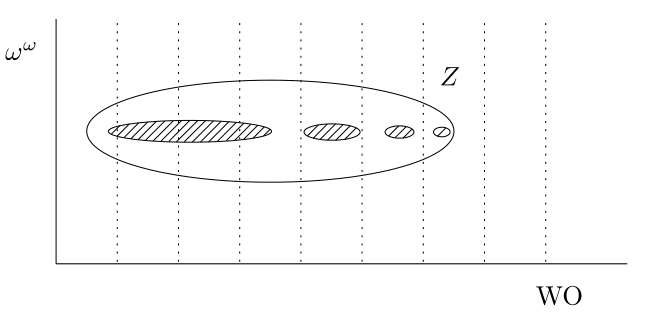
\includegraphics[scale=0.6]{coding1.png}
		\caption{Basic coding.}
	\end{center}
\end{figure}

Here $x_i,y_i<\omega$ and player II wins iff $x\in\wo$ implies that $y$ codes a countable selector $Y\subset Z$ for $Z\cap(\wo_{\leq\alpha_x}\times\r)$. So the idea is that player I challenges player II to play a selector for $Z$ up to $\alpha_x$. These games are now known as 'Solovay games', and the key property of these games is that player I cannot have a winning strategy. The reason for this is that player II has the power to 'take control' of the game, in the following sense. Let $\sigma$ be a winning strategy for player I and define
\eq{
	X:=\{(\sigma*y)_I\mid y\in\r\}.
}

Note that $X$ is $\Sigma^1_1(\sigma)$ and as $\sigma$ is winning, $X\subset\wo$. Then $\b\Sigma^1_1$-Boundedness implies that there is some $\alpha<\omega_1$ such that $X\subset\wo_{<\alpha}$. As $\ac_\omega(\mathbb R)$ holds we can find a selector $Y$ for $Z\cap(\wo_{<\alpha}\times\r)$ -- let $y\in\r$ code $Y$. Then $\sigma*y$ is a win for player I, $\contr$. Thus $\ad$ implies that player II has a winning strategy $\tau$. But then, letting $Y^x$ be the countable selector coded by $(x*\tau)_{II}$ we can set
\eq{
	Z^*:=\bigcup\{Y^x\mid x\in\wo\},
}

which is $\Sigma^1_2(\tau)$ and is a selector for $Z\cap(\wo\times\r)$. With a bit more work the 'moreover' part can be shown. We can now give a proof of Solovay's Theorem.

\theo[Solovay]{
	\label{theo.warmup1}
	Assume $\zf+\ad$. Then
	\eq{
		L(\mathbb R)\models\omega_1^V\text{ is measurable}.
	}
}
\proof{
	To each $S\subset\omega_1$ define a game $\G(S)$ as
	\game{x_0}{y_0}{x_1}{y_1}{x_2}{y_2}{\cdots}{\cdots}

	Here we require that $(x)_i,(y)_i\in\wo$ for every $i<\omega$ and that
	\eq{
		\alpha_{(x)_0}<\alpha_{(y)_0}<\alpha_{(x)_1}<\alpha_{(y)_1}\cdots
	}

	Then player I wins iff $\sup_i\alpha_{(x)_i}\in S$. Define
	\eq{
		\mu:=\{S\subset\omega_1\mid\text{Player I wins }\G(S)\}.
	}

	Clearly $\mu$ is non-principal, is upwards closed and $\ad$ ensures that is has the ultra property. It remains to show that it's normal. Assume not and let $f:\omega_1\to\omega_1$ be regressive such that there's no $\alpha<\omega_1$ such that $\{\xi<\omega_1\mid f(\xi)=\alpha\}\notin\mu$, or equivalently that
	\eq{
		S_\alpha:=\{\xi<\omega_1\mid f(\xi)\neq\alpha\}\in\mu.
	}

	We now aim to recursively construct
	\begin{itemize}
		\item An increasing sequence $\bra{\eta_i\mid i<\omega}$ of countable ordinals;
		\item A sequence of sets of strategies $\bra{X_i\mid i<\omega}$ where $X_i$ consists of winning strategies for player I in $\G(S_\alpha)$ for $\alpha\in[\eta_{i-1},\eta_i)$ where $\eta_{-1}:=0$;
		\item A sequence $\bra{y_i\mid i<\omega}$ of reals such that $y_i$ is legal for player II against any $\sigma\in X_i$ and $\sup_j\alpha_{(y_i)_j}=\sup_i\eta_i$.
	\end{itemize}

	This then means that the $y_i$'s will witness that $f(\eta)\neq\alpha$ for any $\alpha<\eta$, contradicting that $f$ is regressive. Firstly we set
	\eq{
		Z:=\{(x,\sigma)\mid x\in\wo\land\sigma\text{ is winning for player I in }\G(S_\alpha)\}.
	}

	Let $Z^*:=X\cap(\wo\times\r)$ be a selector for $Z\cap(\wo\times\r)$ with $X$ being $\Sigma^1_1(t)$ for some real $t\in\r$, and note that $X\cap(\wo_{\leq\alpha}\times\r)$ is $\bf\Sigma^1_1$ as well. It turns out that we'll need $\dc$ to construct the above $y_i$'s, so to deal with that we jump to $L[t,f]$. Everything is $\bf\Sigma^1_2$ definable and thus by Shoenfield absoluteness it's absolute to this model, so we lose nothing by working there. Now set
	\eq{
		\eta_0&:=\text{any countable ordinal}\\
		X_0&:=\text{proj}_2(X\cap(\wo_{<\eta_0}\times\r))\\
		Y_0&:=\{((\sigma*y)_I)_0\mid\sigma\in X_0\land y\in\r\}\\
		z_0&:=\text{any reals such that }Y_0\subset\wo_{<\alpha_z}.
	}

	where $\eta_0$ and $X_0$ can be seen to satisfy the above conditions. Here we note that $Y_0$ is $\Sigma^1_1(t)$, so that $\bf\Sigma^1_1$-boundedness implies that we can bound $Y_0$ and $z_0$ is one such bound. At the next stage set
	\eq{
		\eta_1:=&\text{any countable ordinal}>\eta_0,\alpha_{z_0}\\
		X_1:=&\text{proj}_2(X\cap(\wo_{[\eta_0,\eta_1)}\times\r))\\
		Y_1:=&\{((\sigma*y)_I)_1\mid \sigma\in X_0\land y\in\r\land (y)_0=z_0\}\\
		&\cup\{((\sigma*y)_I)_0\mid\sigma\in X_1\land y\in\r\}\\
		z_1:=&\text{any real in $\wo$ such that }Y_1\subset\wo_{<\alpha_z},
	}

	and for general $n<\omega$ we put
	\eq{
		\eta_{n+1}:=&\text{any countable ordinal}>\eta_n,\alpha_{z_n}\\
		X_{n+1}:=&\text{proj}_2(X\cap(\wo_{[\eta_n,\eta_{n+1})}\times\r))\\
		Y_{n+1}:=&\bigcup_{k\leq n+1}\{((\sigma*y)_I)_k\mid\sigma\in X_{n+1-k}\land y\in\r\land\forall i<k:(y)_i=z_{i+n+1-k}\}\\
		z_{n+1}:=&\text{any real in $\wo$ such that }Y_{n+1}\subset\wo_{<\alpha_z}.
	}

	All the $\eta$'s and $X$'s satisfy our conditions, so we now need to construct our $y$ sequence. To do that use $\dc$ to define $y_k\in\r$ such that $(y_k)_i=z_{i+k}$ for every $i<\omega$. Then we see that $\sup_i\alpha_{(y_k)_i}=\sup_i\alpha_{z_{i+k}}=\sup_i\eta_i$, which deals with one of the conditions of the $y$'s.
	
	\qquad We also claim that $y_k$ is a legal play for player II against any $\sigma\in X_k$, as this can be seen witnessed by the $(k+1)$'st components of $Y_n$ for $n\geq k$. By definition $(y_k)_i=z_{i+k}\in\wo$ for all $k,i<\omega$, so the first rule is satisfied. As for the second rule, let's for simplicity focus on the case $k=1$. We need to show that
	\eq{
		\alpha_{(x)_0}<\alpha_{(y_1)_0}<\alpha_{(x)_1}<\alpha_{(y_1)_1}<\cdots
	}

	where $x:=(\sigma*y_1)_I$, for an arbitrary $\sigma\in X_1$. Since $\alpha_{(y_1)_0}=\alpha_{z_1}$ and $(x)_0\in Y_1$ by definition of $Y_1$, we get that $\alpha_{(x)_0}<\alpha_{(y_1)_1}$ by definition of $z_1$. Next, $\alpha_{(y_1)_0}<\alpha_{(x)_1}$ simply because $\sigma$ is winning. To take one last example, $(y_1)_1=z_2$ and $\alpha_{(x)_1}\in Y_2$ (it lies in the first component since $(y_1)_0=z_1$), so $\alpha_{(x)_1}<\alpha_{(y_1)_1}$.
}

This finishes the first warm-up.

\pagebreak
\section{Second warm-up: measurability of $(\bf\delta^2_1)^{L(\mathbb R)}$}

The ordinal $\bf\delta^k_m$ for $k,m<\omega$ is defined as the least ordinal $\alpha$ such that there is a $\bf\Delta^k_m$ surjection $f:\r\to\alpha$, or equivalently, the least ordinal $\alpha$ such that there is a $\bf\Delta^k_m$ pre-wellordering of $\r$. In our first warm-up we showed that $\omega_1^V$ is measurable in $L(\mathbb R)$, and $\omega_1^V$ turns out to be equal to $(\bf\delta^1_1)^{L(\mathbb R)}$, so all we're doing is upping the complexity of our surjections/pre-wellorderings. Just to make notation a bit simpler,

\begin{center}
\framebox{\textbf{We assume $V=L(\mathbb R)$.}}
\end{center}

There is something special about $\bf\delta^2_1$, in that it turns out to be \textbf{the least stable}, meaning that it's the least ordinal $\alpha$ such that $L_\alpha(\mathbb R)\prec_{\Sigma_1}L(\mathbb R)$ -- so just by talking about existence claims of sets of reals, we suddenly get \textit{all} existence claims. The proof of the measurability of $\bf\delta^2_1$ is going to be a carbon copy of the proof of the measurability of $\bf\delta^1_1$ -- all we need to do is replace a few notions. 

\qquad As the replacement for $\wo$ we pick a universal $\Sigma^2_1$ set $\U$; i.e. a $\Sigma^2_1$ set $\U\subset\r\times\r$ such that whenever $A\subset\r$ is $\bf\Sigma^1_2$ then there is a real $x\in\r$ satisfying $A=\U_x:=\{y\in\r\mid (x,y)\in\U\}$. We now want to stratify $\U$ as we did with $\wo$ using the $\alpha_x$'s -- these analogues will be ordinals $\delta_x<\bf\delta^2_1$ cofinal in $\bf\delta^2_1$. The analogy is shown in Figure \ref{fig.analogy}. Towards defining the $\delta_x$'s, firstly define the theory $T_0$ given as
\eq{
	T_0:=\zf^-+"\p(\omega)\text{ exists}"+\ac_\omega(\mathbb R).
}

\renewcommand{\arraystretch}{1.5}
\begin{figure}
	\label{fig.analogy}
\begin{center}
	\begin{tabular}{c | c}
		\hline$\bf\delta^1_1$ & $\bf\delta^2_1$\\[3pt]\hline
	$\wo$ & $\U$\\
	$\bf\delta^1_1$-many $\alpha_x$'s & $\bf\delta^2_1$-many $\delta_x$'s\\
	$\bf\Sigma^1_1$-boundedness & $\bf\Delta^2_1$-boundedness\\
	$\bf\Sigma^1_2$-coding & $\bf\Sigma^2_1$-coding\\\hline
\end{tabular}
\end{center}
\caption{The analogy between the $\bf\delta^1_1$-case and the $\bf\delta^2_1$-case.}
\end{figure}

We're going to need a few facts about $T_0$. First of all, we take it for granted that $L_\Theta(\mathbb R)\models T_0$. This means that given any $\xi<\bf\delta^2_1$ it holds that
\eq{
	L(\mathbb R)\models\exists\alpha(L_\alpha(\mathbb R)\models T_0\land \alpha>\xi).
}

Since $\bf\delta^2_1$ is the least stable this statement reflects down to $L_{\bf\delta^2_1}(\mathbb R)$, so we get that there is some $\alpha\in(\xi,\bf\delta^2_1)$ such that $L_\alpha(\mathbb R)\models T_0$. We've proved the following.

\qprop{
	There are cofinally many $\alpha<\bf\delta^2_1$ such that $L_\alpha(\mathbb R)\models T_0$.
}

Now, given $(y,z)\in\U$ we let $\Theta_{(y,z)}$ be the least ordinal such that $L_{\Theta_{(y,z)}}(\mathbb R)\models T_0$ and $(y,z)\in\U^{L_{\Theta_{(y,z)}}(\mathbb R)}$. We know that such an ordinal exists and that it's below $\bf\delta^2_1$, by the above proposition. We then set $\delta_{(y,z)}:=(\bf\delta^2_1)^{L_{\Theta_{(y,z)}}(\mathbb R)}$. Identifying $\r\times\r$ with $\r$ via a recursive bijection, we can think of $\U$ as being a set of reals, so for each $x\in\U$ we get an ordinal $\delta_x$.

\prop{
	The $\delta_x$'s are cofinal in $\bf\delta^2_1$.
}
\proof{
	Let $\xi<\bf\delta^2_1$ be arbitrary. By definition we can find some $\bf\Delta^2_1$ pre-wellordering of $\r$, which we can code up as a subset $A\subset\r$. Then as both $A$ and $\lnot A$ are $\bf\Sigma^2_1$ we can find $x,y\in\r$ such that $A=\U_x$ and $\lnot A=\U_y$. Then since $L(\mathbb R)\models\U_x=\lnot\U_y$ there's some $\beta<\bf\delta^2_1$ such that $L_\beta(\mathbb R)\models\U_x=\lnot\U_y$, using again that $\bf\delta^2_1$ is the least stable. But as $\U_x^{L_\beta(\mathbb R)}\subset\U_x$ and $\lnot\U_y^{L_\beta(\mathbb R)}\subset\lnot\U_y$ we in fact get that $\U_x^{L_\beta(\mathbb R)}=A$. But then pick some $z\in\U-\U^{L_\beta(\mathbb R)}$ and note that $A\in L_{\Theta_z}(\mathbb R)$ and that the ordertype of $A$, i.e. $\xi$, can be computed inside $L_{\Theta_z}$, so that $\xi<({\bf\delta^2_1})^{L_{\Theta_z}(\mathbb R)}=\delta_z$.
}

This shows that we now have an analogous stratification of $\U$ as we had with $\wo$. As for the boundedness, we have the following.

\lemm[Moschovakis]{
	Assume $\zf+\ac_\omega(\mathbb R)+V=L(\mathbb R)$ and let $X\subset\U$ be $\bf\Delta^2_1$. Then there's some $x\in\U$ such that $X\subset\U_{<\delta_x}$.
}
\proof{
	Just as in the above proof we can find some $y\in\r$ and $\beta<\bf\delta^2_1$ such that $X=\U_y^{L_\beta(\mathbb R)}$. Pick any $\gamma>\beta$ such that $L_\gamma(\mathbb R)\models T_0$. Then if we take any $z\in X$, $\Theta_z\leq\gamma$, so that $\delta_z<\gamma$. If we then just pick any $x\in\U$ with $\delta_x>\gamma$, this $x$ works.
}

Moschovakis also supplies us with the following analogous coding lemma, whose proof I won't supply here.

\qlemm[Moschovakis]{
	Assume $\zf+\ad$ and let $Z\subset\U\times\r$. Then there is a $\bf\Sigma^2_1$ selector $Z^*\subset Z$ for $Z$.
}

Now that we have all the ingredients that we need, the \textit{exact} same proof as in our first warm-up goes through. The only difference is that to build the $z$-sequence we have to use $\dc$, as we can't just jump to $L$ as we did there. This use of $\dc$ can be circumvented, but we won't go into that here.

\theo[Moschovakis]{
	Assume $\zf+\dc+\ad$. Then
	\eq{
		L(\mathbb R)\models\bf\delta^2_1\text{ is measurable}.
	}
}

This finishes the second warm-up. Now, let's get started with the actual proof.


\section{Ideas used to show $\Theta$ is Woodin}

We're trying to show that $\Theta$ is Woodin, so given any $A\subset\Theta$ we need to find some $\kappa<\Theta$ which is $A$-reflecting. We're only going to focus on the case where $A=\emptyset$ here, as it turns out that the general case is not too hard when we've shown this, as everything is just relativised to $A$. The given $\kappa$ that we're interested in is $\bf\delta^2_1$. In other words, we need to show that given any $\lambda<\Theta$ we can find an elementary embedding $j:V\to\M$ with $\crit j=\bf\delta^2_1$, $j(\bf\delta^2_1)>\lambda$ and $V_\lambda\subset\M$.

\qquad The main new idea is that we have a \textit{reflection phenomenon} at $\bf\delta^2_1$: there exists a function $F:\bf\delta^2_1\to L_{\bf\delta^2_1}(\mathbb R)$ such that

\begin{quotation}
	Given any $X\in L(\mathbb R)\cap\od^{L(\mathbb R)}$, $z\in\r$ and $\Sigma_1$ formula $\varphi$, if
	\eq{
		L(\mathbb R)\models\varphi[z,X,\bf\delta^2_1,\mathbb R]
	}

	then there's a $\delta<\bf\delta^2_1$ such that
	\eq{
		L(\mathbb R)\models\varphi[z,F(\delta),\delta,\mathbb R].
	}
\end{quotation}

This $F$ is constructed analogously to $\diamondsuit$-sequences in $L$, i.e. defining it by least counterexample. Now for any such $X$ let $\U_X$ be a universal $\Sigma_1^{L(\mathbb R)}(\{X,\bf\delta^2_1,\mathbb R\})$ set and for each $\delta<\bf\delta^2_1$ let $\U_\delta$ be a universal $\Sigma_1^{L(\mathbb R)}(\{F(\delta),\delta,\mathbb R\})$ set, obtained by using the same definition as $\U_X$ -- both $\U_X$ and $\U_\delta$ are treated as sets of reals, just as we did with $\U$.

\qquad Now, given any $\Sigma_1$ formula $\varphi$ and $y\in\r$ there is a real $z_{\varphi,y}$ such that
\eq{
	z_{\varphi,y}\in\U_X\qquad\text{iff}\qquad L(\mathbb R)\models\varphi[y,X,\bf\delta^2_1,\mathbb R].
}

To see this, the set of $y$'s defined by the above right-hand side is a $\Sigma_1^{L(\mathbb R)}(\{X,\bf\delta^2_1,\mathbb R\})$ set, so it's $(\U_X)_x$ for some $x\in\r$. But then we just take $z_{\varphi,y}:=\bra{x,y}$. We say that $z_{\varphi,y}$ \textbf{certifies} that $\varphi$ holds of $y$. Note that by the way that we picked the $\U_\delta$'s, if $z_{\varphi,y}\in\U_\delta$ we get that $L(\mathbb R)\models\varphi[y,F(\delta),\delta,\mathbb R]$. The reflection phenomenon can then be stated as $\U_X\subset\bigcup_{\delta<\bf\delta^2_1}\U_\delta$.

\qquad We now get to define the measure on $\bf\delta^2_1$. Let $\lambda<\Theta$ be arbitrary, let $\leq_\lambda$ be an $\od$ pre-wellordering of $\r$, set $X:=(\leq_\lambda,\lambda)$ and for each $S\subset\bf\delta^2_1$ define the game $G^X(S)$ as
\game{x_0}{y_0}{x_1}{y_1}{x_2}{y_2}{\cdots}{\cdots}

We got only one rule in this game, which is that $(x)_i,(y)_i\in\U_X$ for every $i<\omega$. In that case the statement
\eq{
	\forall i<\omega:(x)_i\in\U_X\land (y)_i\in\U_X
}

is a $\Sigma_1^{L(\mathbb R)}(\{X,\bf\delta^2_1,\mathbb R\})$ statement, so it reflects and there is some $\delta<\bf\delta^2_1$ such that $(x)_i,(y)_i\in\U_\delta$ for every $i<\omega$. We then define that player I wins iff $\delta\in S$. Just as in the $\bf\delta^1_1$ case we define
\eq{
	\mu_X:=\{S\subset{\bf\delta^2_1}\mid\text{Player I wins }G^X(S)\}.
}

We also define for $z\in\U_X$ the sets $S_z:=\{\delta<\bf\delta^2_1\mid z\in\U_\delta\}$ and let
\eq{
	\mathcal F_X:=\{S\subset{\bf\delta^2_1}\mid\exists z\in\U_X:S_z\subset S\}
}

be the \textbf{reflection filter}. Note that $\mathcal F_X\subset\mu_X$, as player I can win $G^X(S_z)$ by playing $x_i$ such that $(x)_i\in\U_X$ for every $i<\omega$ and that $(x)_i=z$ for some $i<\omega$. It turns out that the reflection filter is indeed an $\aleph_1$-complete filter, and it's a key tool in showing that sets lie in $\mu_X$.

\qquad We do also have an analogous coding lemma in this case, where this coding lemma subsumes the previous two. Let $\U^{(2)}(P)\subset(\r)^3$ be a universal $\Sigma_1^{L(\mathbb R)}(P)$ set.

\qtheo[Uniform coding; Moschovakis]{
	Assume $\zf+\ad$. Suppose $X\subset\r$ and $\pi:X\to\on$. Let $Z\subset X\times\r$. Then there exists an $e\in\r$ such that for every $a\in X$,
	\begin{enumerate}
		\item $\U^{(2)}_e(Q_{<a},Q_a)\subset Z\cap(Q_a\times\r)$;
		\item $\U^{(2)}_e(Q_{<a},Q_a)\neq\emptyset$ iff $Z\cap(Q_a\times\r)\neq\emptyset$,
	\end{enumerate}

	where $Q_{<a}:=\{b\in X\mid\pi(b)<\pi(a)\}$ and $Q_a:=\{b\in X\mid \pi(b)=\pi(a)\}$.
}

See Figure \ref{fig.coding2} for an illustration of the above uniform coding. To see the previous coding lemmas as a special case of this theorem, take $Z^*:=\bigcup_{a\in X}\U^{(2)}_e(Q_{<a},Q_a)\subset Z$, which is $\Sigma_1(Q_{<a},Q_a)$. In the $\wo$ case the $Q_a$ and $Q_{<a}$ are $\bf\Sigma^1_2$, so that $Z^*$ is $\bf\Sigma^1_2$ as well. In the $\U$ case we analogously get that $Z^*$ is $\bf\Sigma^2_1$.

\begin{figure}
	\label{fig.coding2}
	\begin{center}
		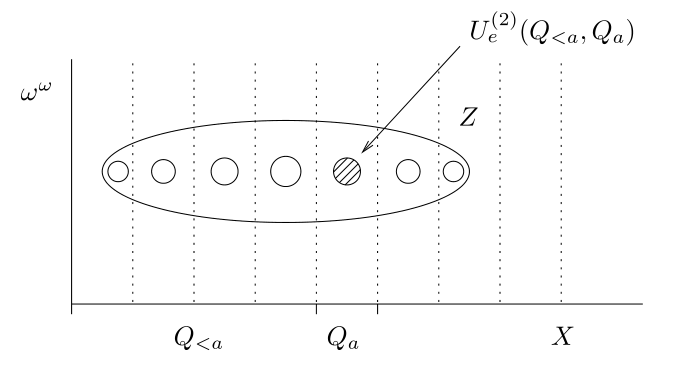
\includegraphics[scale=0.5]{coding2.png}
		\caption{Uniform coding.}
	\end{center}
\end{figure}

Like in the $\bf\delta^1_1$ case we easily see that $\mu_X$ is non-principal, is upwards closed and satisfies the ultra property. It remains to see that $\mu_X$ is $\bf\delta^2_1$-complete and that it witnesses that the associated ultrapower embedding is $\lambda$-strong. We will define a notion called \textit{strongly normal}, which will imply all these three things. To define this, first let $Q_\alpha^{\bf\delta^2_1}$ be the $\alpha$'th component of $\leq_\lambda$ and setting
\eq{
	S_0:=\{\delta<{\bf\delta^2_1}\mid& F(\delta)=(\leq_\delta,\lambda_\delta)\land"\leq_\delta\text{ is a pre-wellordering of $\r$ of length $\lambda_\delta$}"\\
		&\land L_{\lambda_\delta}(\mathbb R)\models T_0\},
}

let $Q_\alpha^\delta$ to be the $\alpha$'th component of $\leq_\delta$. For $\delta\in S_0$ and $t\in\r$ let $\alpha_t^\delta$ be the unique $\alpha$ such that $t\in Q_\alpha^\delta$ and define $f_t:S_0\to\bf\delta^2_1$ as $f_t(\delta):=\alpha_t^\delta$.

\defi{
	$\mu_X$ is \textbf{strongly normal} if whenever $f:S_0\to\bf\delta^2_1$ satisfies $f(\delta)<\lambda_\delta$ for $\mu_X$-many $\delta$, there is some $t\in\r$ such that $f(\delta)=f_t(\delta)$ for $\mu_X$-many $\delta$.
}

\prop{
If $\mu_X$ is strongly normal then $\mu_X$ is also normal.
}
\proof{
	If $f(\delta)<\delta$ for $\mu_X$-many $\delta$ then (since $\delta<\lambda_\delta$ for $\mu_X$-many $\delta$) by strong normality there is a $t\in\r$ such that
	\eq{
		\forall^{\mu_X}\delta:f_t(\delta)=f(\delta).
	}

	Letting $\beta$ be such that $t\in Q_\beta^{\bf\delta^2_1}$ we get that $\beta<\bf\delta^2_1$, as otherwise by reflection we get that $f_t(\delta)\geq\delta$ for $\mu_X$-many $\delta$, contradicting that $f(\delta)<\delta$ for $\mu_X$-many $\delta$. It thus holds that $f(\delta)=\beta$ for $\mu_X$-many $\delta$, making $\mu_X$ normal.
}

Now the key thing is that strong normality implies that $[f_t]_{\mu_X}$ collapses to $|t|_{\leq_\lambda}$ in the ultrapower (so that we can think of them as being equal). Here $|t|_{\leq_\lambda}$ is the rank of $t$ with respect to $\leq_\lambda$. This shows that, given that $\mu_X$ is strongly normal, $\lambda<j_X({\bf\delta^2_1})$ as $[f_t]<j_X({\bf\delta^2_1})$ for every $t\in\r$.

\qquad To show that $\p(\lambda)\cap\hod^{L(\mathbb R)}\subset\ult(V,\mu_X)$, let $A\subset\lambda$ with $A\in\hod^{L(\mathbb R)}$. By uniform coding there is an $e(A)\in\r$ such that for every $\alpha<\lambda$,
\eq{
	\U^{(2)}_{e(A)}(Q_{<\alpha}^{\bf\delta^2_1},Q_\alpha^{\bf\delta^2_1})\neq\emptyset\qquad\text{iff}\qquad\alpha\in A,
}

so set $A^\delta:=\{\alpha<\lambda_\delta\mid\U^{(2)}_{e(A)}(Q_{<\alpha}^\delta,Q_\alpha^\delta)\neq\emptyset\}$. Assume that we've picked our $\lambda$ such that $L_\lambda(\mathbb R)\prec L_\Theta(\mathbb R)$ and ${\bf\delta^2_1}<\lambda$, as it can be shown that there are arbitrarily large $\lambda$ satisfying these two conditions. The reason for this is that it turns out that such $\lambda$ satisfy $\hod^{L(\mathbb R)}\cap V_\lambda=\hod^{L_\lambda(\mathbb R)}$, so that
\eq{
	\{\alpha<\lambda\mid\U^{(2)}_{e(A)}(Q_{<\alpha}^{\bf\delta^2_1},Q_\alpha^{\bf\delta^2_1})\neq\emptyset\}\in\hod^{L(\mathbb R)}
}

is a true $\Sigma_1^{L(\mathbb R)}$ statement about $X$, $\mathbb R$ and $e(A)$. This means that there's an $S\in\mathcal F_X$ such that for every $\delta\in S$, $A^\delta\in\hod^{L(\mathbb R)}$. Now set $h_A:S\to\hod^{L(\mathbb R)}$ to be $h_A(\delta):=A^\delta$. Then
\eq{
	|t|_{\leq_\lambda}\in A\qquad &\text{iff}\qquad\{\delta<{\bf\delta^2_1}\mid f_t(\delta)\in A^\delta\}\in\mu_X\\
	&\text{iff}\qquad [f_t]\in[h_A],
}

so since $[f_t]=|t|_{\leq_\lambda}$, assuming strong normality, we get $A=[h_A]\in\ult(V,\mu_X)$. The first equivalence above is by reflection.

\qquad This shows that if $\mu_X$ is strongly normal then it's also $\lambda$-strong, making $\bf\delta^2_1$ $\emptyset$-reflecting. The proof of strong normality is a technical tour de force and will be omitted here, see \cite{KoellnerWoodin}. The "final step" is then to show that given any $A\subset\Theta$ we can find some $\kappa<\Theta$ which is $A$-reflecting. This is done in an analogous fashion, where the $\kappa$ in question is taken to be the "least $A$-stable", i.e. the least $\alpha$ such that $L_\alpha(\mathbb R)[A\cap\alpha]\prec_{\Sigma_1} L_\Theta(\mathbb R)[A]$. It turns out that we also get an analogous reflection phenomenon, so that by essentially the same strategy, $\mu_X^A$, the relativised version of $\mu_X$, is $\lambda$-$A$-strong, finishing the proof.

\bibliographystyle{apalike}
\nocite{*}
\bibliography{bib}

\end{document}
